%\title{University of Bristol Thesis Template}
\RequirePackage[l2tabu]{nag}		% Warns for incorrect (obsolete) LaTeX usage
%
%
% File: memoirthesis.tex
% Author: Victor Brena
% Description: Contains the thesis template using memoir class,
% which is mainly based on book class but permits better control of 
% chapter styles for example. This template is an adaptation and 
% modification of Oscar's.
% 
% Memoir is a flexible class for typesetting poetry, fiction, 
% non-fiction and mathematical works as books, reports, articles or
% manuscripts. CTAN repository is found at:
% http://www.ctan.org/tex-archive/macros/latex/contrib/memoir/
%
%
% UoB guidelines for thesis presentation were found at:
% http://www.bris.ac.uk/esu/pg/pgrcop11-12topic.pdf#page=49
%
% UoB guidelines:
%
% The dissertation must be printed on A4 white paper. Paper up to A3 may be used
% for maps, plans, diagrams and illustrative material. Pages (apart from the
% preliminary pages) should normally be double-sided.
%
% Memoir class loads useful packages by default (see manual).
\documentclass[a4paper,11pt,leqno,openbib,oldfontcommands]{memoir} %add 'draft' to turn draft option on (see below)
%
%
% Adding metadata:
\usepackage[table,x11names]{xcolor}
\usepackage{caption}
\usepackage{subcaption}
\usepackage{datetime}
\usepackage{ifpdf}
\ifpdf
\pdfinfo{
   /Author (Shivan Ramdhanie)
   /Title (MSc. Thesis)
   /Keywords (One; Two;Three)
   /CreationDate (D:\pdfdate)
}
\fi
% When draft option is on. 
\ifdraftdoc 
	\usepackage{draftwatermark}				%Sets watermarks up.
	\SetWatermarkScale{0.3}
	\SetWatermarkText{\bf Draft: \today}
\fi
%
% Declare figure/table as a subfloat.
\newsubfloat{figure}
\newsubfloat{table}
% Better page layout for A4 paper, see memoir manual.
\settrimmedsize{297mm}{210mm}{*}
\setlength{\trimtop}{0pt} 
\setlength{\trimedge}{\stockwidth} 
\addtolength{\trimedge}{-\paperwidth} 
\settypeblocksize{634pt}{448.13pt}{*} 
\setulmargins{4cm}{*}{*} 
\setlrmargins{*}{*}{1.5} 
\setmarginnotes{17pt}{51pt}{\onelineskip} 
\setheadfoot{\onelineskip}{2\onelineskip} 
\setheaderspaces{*}{2\onelineskip}{*} 
\checkandfixthelayout
%
\frenchspacing
% Font with math support: New Century Schoolbook
\usepackage{fouriernc}
\usepackage[T1]{fontenc}
%
% UoB guidelines:
%
% Text should be in double or 1.5 line spacing, and font size should be
% chosen to ensure clarity and legibility for the main text and for any
% quotations and footnotes. Margins should allow for eventual hard binding.
%
% Note: This is automatically set by memoir class. Nevertheless \OnehalfSpacing 
% enables double spacing but leaves single spaced for captions for instance. 
\OnehalfSpacing 
%
% Sets numbering division level
\setsecnumdepth{subsection} 
\maxsecnumdepth{subsubsection}
%
% Chapter style (taken and slightly modified from Lars Madsen Memoir Chapter 
% Styles document
\usepackage{calc,soul,fourier}
\makeatletter 
\newlength\dlf@normtxtw 
\setlength\dlf@normtxtw{\textwidth} 
\newsavebox{\feline@chapter} 
\newcommand\feline@chapter@marker[1][4cm]{%
	\sbox\feline@chapter{% 
		\resizebox{!}{#1}{\fboxsep=1pt%
			\colorbox{gray}{\color{white}\thechapter}% 
		}}%
		\rotatebox{90}{% 
			\resizebox{%
				\heightof{\usebox{\feline@chapter}}+\depthof{\usebox{\feline@chapter}}}% 
			{!}{\scshape\so\@chapapp}}\quad%
		\raisebox{\depthof{\usebox{\feline@chapter}}}{\usebox{\feline@chapter}}%
} 
\newcommand\feline@chm[1][4cm]{%
	\sbox\feline@chapter{\feline@chapter@marker[#1]}% 
	\makebox[0pt][c]{% aka \rlap
		\makebox[1cm][r]{\usebox\feline@chapter}%
	}}
\makechapterstyle{daleifmodif}{
	\renewcommand\chapnamefont{\normalfont\Large\scshape\raggedleft\so} 
	\renewcommand\chaptitlefont{\normalfont\Large\bfseries\scshape} 
	\renewcommand\chapternamenum{} \renewcommand\printchaptername{} 
	\renewcommand\printchapternum{\null\hfill\feline@chm[2.5cm]\par} 
	\renewcommand\afterchapternum{\par\vskip\midchapskip} 
	\renewcommand\printchaptertitle[1]{\color{gray}\chaptitlefont\raggedleft ##1\par}
} 
\makeatother 
\chapterstyle{daleifmodif}
%
% UoB guidelines:
%
% The pages should be numbered consecutively at the bottom centre of the
% page.
\makepagestyle{myvf} 
\makeoddfoot{myvf}{}{\thepage}{} 
\makeevenfoot{myvf}{}{\thepage}{} 
\makeheadrule{myvf}{\textwidth}{\normalrulethickness} 
\makeevenhead{myvf}{\small\textsc{\leftmark}}{}{} 
\makeoddhead{myvf}{}{}{\small\textsc{\rightmark}}
\pagestyle{myvf}
%
% Oscar's command (it works):
% Fills blank pages until next odd-numbered page. Used to emulate single-sided
% frontmatter. This will work for title, abstract and declaration. Though the
% contents sections will each start on an odd-numbered page they will
% spill over onto the even-numbered pages if extending beyond one page
% (hopefully, this is ok).
\newcommand{\clearemptydoublepage}{\newpage{\thispagestyle{empty}\cleardoublepage}}
%
%
% Creates indexes for Table of Contents, List of Figures, List of Tables and Index
\makeindex
% \printglossaries below creates a list of abbreviations. \gls and related
% commands are then used throughout the text, so that latex can automatically
% keep track of which abbreviations have already been defined in the text.
%
% The import command enables each chapter tex file to use relative paths when
% accessing supplementary files. For example, to include
% chapters/brewing/images/figure1.png from chapters/brewing/brewing.tex we can
% use
% \includegraphics{images/figure1}
% instead of
% \includegraphics{chapters/brewing/images/figure1}
\usepackage{import}

% Add other packages needed for chapters here. For example:
\usepackage{lipsum}					%Needed to create dummy text
\usepackage{amsfonts} 					%Calls Amer. Math. Soc. (AMS) fonts
\usepackage[centertags]{amsmath}			%Writes maths centred down
\usepackage{stmaryrd}					%New AMS symbols
\usepackage{amssymb}					%Calls AMS symbols
\usepackage{amsthm}					%Calls AMS theorem environment
\usepackage{newlfont}					%Helpful package for fonts and symbols
\usepackage{layouts}					%Layout diagrams
\usepackage{graphicx}					%Calls figure environment
\usepackage{longtable,rotating}			%Long tab environments including rotation. 
\usepackage[utf8]{inputenc}			%Needed to encode non-english characters 
									%directly for mac
\usepackage{colortbl}					%Makes coloured tables
\usepackage{wasysym}					%More math symbols
\usepackage{mathrsfs}					%Even more math symbols
\usepackage{float}						%Helps to place figures, tables, etc. 
\usepackage{verbatim}					%Permits pre-formated text insertion
\usepackage{upgreek }					%Calls other kind of greek alphabet
\usepackage{latexsym}					%Extra symbols
%\usepackage[square,numbers,
%		     sort&compress]{natbib}		%Calls bibliography commands
\usepackage{natbib}
\usepackage{url}						%Supports url commands
% \usepackage{etex}						%eTeXÕs extended support for counters
% \usepackage{fixltx2e}					%Eliminates some in felicities of the 
									%original LaTeX kernel
\usepackage[spanish,english]{babel}		%For languages characters and hyphenation
\usepackage{color}                    				%Creates coloured text and background
\usepackage[colorlinks=true,
		     allcolors=black]{hyperref}              %Creates hyperlinks in cross references
\usepackage{memhfixc}					%Must be used on memoir document 
									%class after hyperref
\usepackage{enumerate}					%For enumeration counter
\usepackage{footnote}					%For footnotes
\usepackage{microtype}					%Makes pdf look better.
\usepackage{rotfloat}					%For rotating and float environments as tables, 
									%figures, etc. 
\usepackage{alltt}						%LaTeX commands are not disabled in 
									%verbatim-like environment
\usepackage[version=0.96]{pgf}			%PGF/TikZ is a tandem of languages for producing vector graphics from a
\usepackage{tikz}						%geometric/algebraic description.
\usetikzlibrary{arrows,shapes,snakes,
		       automata,backgrounds,
		       petri,topaths}				%To use diverse features from tikz		
%
%Reduce widows  (the last line of a paragraph at the start of a page) and orphans 
% (the first line of paragraph at the end of a page)
\widowpenalty=1000
\clubpenalty=1000
%
% New command definitions for my thesis
%
\newcommand{\keywords}[1]{\par\noindent{\small{\bf Keywords:} #1}} %Defines keywords small section
\newcommand{\parcial}[2]{\frac{\partial#1}{\partial#2}}                             %Defines a partial operator
\newcommand{\vectorr}[1]{\mathbf{#1}}                                                        %Defines a bold vector
\newcommand{\vecol}[2]{\left(                                                                         %Defines a column vector
	\begin{array}{c} 
		\displaystyle#1 \\
		\displaystyle#2
	\end{array}\right)}
\newcommand{\mados}[4]{\left(                                                                       %Defines a 2x2 matrix
	\begin{array}{cc}
		\displaystyle#1 &\displaystyle #2 \\
		\displaystyle#3 & \displaystyle#4
	\end{array}\right)}
\newcommand{\pgftextcircled}[1]{                                                                    %Defines encircled text
    \setbox0=\hbox{#1}%
    \dimen0\wd0%
    \divide\dimen0 by 2%
    \begin{tikzpicture}[baseline=(a.base)]%
        \useasboundingbox (-\the\dimen0,0pt) rectangle (\the\dimen0,1pt);
        \node[circle,draw,outer sep=0pt,inner sep=0.1ex] (a) {#1};
    \end{tikzpicture}
}
\newcommand{\range}[1]{\textnormal{range }#1}                                             %Defines range operator
\newcommand{\innerp}[2]{\left\langle#1,#2\right\rangle}                                 %Defines inner product
\newcommand{\prom}[1]{\left\langle#1\right\rangle}                                         %Defines average operator
\newcommand{\tra}[1]{\textnormal{tra} \: #1}                                                       %Defines trace operator
\newcommand{\sign}[1]{\textnormal{sign\,}#1}                                                   %Defines sign operator
\newcommand{\sech}[1]{\textnormal{sech} #1}                                                  %Defines sech
\newcommand{\diag}[1]{\textnormal{diag} #1}                                                    %Defines diag operator
\newcommand{\arcsech}[1]{\textnormal{arcsech} #1}                                       %Defines arcsech
\newcommand{\arctanh}[1]{\textnormal{arctanh} #1}                                         %Defines arctanh
%Change tombstone symbol
\newcommand{\blackged}{\hfill$\blacksquare$}
\newcommand{\whiteged}{\hfill$\square$}
\newcounter{proofcount}
\renewenvironment{proof}[1][\proofname.]{\par
 \ifnum \theproofcount>0 \pushQED{\whiteged} \else \pushQED{\blackged} \fi%
 \refstepcounter{proofcount}
 \normalfont 
 \trivlist
 \item[\hskip\labelsep
       \itshape
   {\bf\em #1}]\ignorespaces
}{%
 \addtocounter{proofcount}{-1}
 \popQED\endtrivlist
}
%
%
% New definition of square root:
% it renames \sqrt as \oldsqrt
\let\oldsqrt\sqrt
% it defines the new \sqrt in terms of the old one
\def\sqrt{\mathpalette\DHLhksqrt}
\def\DHLhksqrt#1#2{%
\setbox0=\hbox{$#1\oldsqrt{#2\,}$}\dimen0=\ht0
\advance\dimen0-0.2\ht0
\setbox2=\hbox{\vrule height\ht0 depth -\dimen0}%
{\box0\lower0.4pt\box2}}
%
% My caption style
\newcommand{\mycaption}[2][\@empty]{
	\captionnamefont{\scshape} 
	\changecaptionwidth
	\captionwidth{0.9\linewidth}
	\captiondelim{.\:} 
	\indentcaption{0.75cm}
	\captionstyle[\centering]{}
	\setlength{\belowcaptionskip}{10pt}
	\ifx \@empty#1 \caption{#2}\else \caption[#1]{#2}
}
%
% My subcaption style
\newcommand{\mysubcaption}[2][\@empty]{
	\subcaptionsize{\small}
	\hangsubcaption
	\subcaptionlabelfont{\rmfamily}
	\sidecapstyle{\raggedright}
	\setlength{\belowcaptionskip}{10pt}
	\ifx \@empty#1 \subcaption{#2}\else \subcaption[#1]{#2}
}
%
%An initial of the very first character of the content
\usepackage{lettrine}
\newcommand{\initial}[1]{%
	\lettrine[lines=3,lhang=0.33,nindent=0em]{
		\color{gray}
     		{\textsc{#1}}}{}}
%
% Theorem styles used in my thesis
%
\theoremstyle{plain}
\newtheorem{theo}{Theorem}[chapter]
\theoremstyle{plain}
\newtheorem{prop}{Proposition}[chapter]
\theoremstyle{plain}
\theoremstyle{definition}
\newtheorem{dfn}{Definition}[chapter]
\theoremstyle{plain}
\newtheorem{lema}{Lemma}[chapter]
\theoremstyle{plain}
\newtheorem{cor}{Corollary}[chapter]
\theoremstyle{plain}
\newtheorem{resu}{Result}[chapter]
%
% Hyphenation for some words
%
\hyphenation{res-pec-tively}
\hyphenation{mono-ti-ca-lly}
\hyphenation{hypo-the-sis}
\hyphenation{para-me-ters}
\hyphenation{sol-va-bi-li-ty}
%
%

\graphicspath{ {./images/} }

\definecolor{LightGreen}{rgb}{.565, .933, .565}

\begin{document}
% UoB guidlines:
%
% Preliminary pages
% 
% The five preliminary pages must be the Title Page, Abstract, Dedication
% and Acknowledgements, Author's Declaration and Table of Contents.
% These should be single-sided.
% 
% Table of contents, list of tables and illustrative material
% 
% The table of contents must list, with page numbers, all chapters,
 % sections and subsections, the list of references, bibliography, list of
% abbreviations and appendices. The list of tables and illustrations
% should follow the table of contents, listing with page numbers the
% tables, photographs, diagrams, etc., in the order in which they appear
% in the text.
% 
\frontmatter
\pagenumbering{roman}
%
%
% File: Title.tex
% Author: V?ctor Bre?a-Medina
% Description: Contains the title page
%
% UoB guidelines:
% 
% At the top of the title page, within the margins, the dissertation should give the title and, if 
% necessary, sub-title and volume number. If the dissertation is in a language other than English, the 
% title must be given in that language and in English. The full name of the author should be in the 
% centre of the page. At the bottom centre should be the words ?A dissertation submitted to the 
% University of Bristol in accordance with the requirements for award of the degree of ? in the 
% Faculty of ...?, with the name of the school and month and year of submission. The word count of 
% the dissertation (text only) should be entered at the bottom right-hand side of the page.
%
%
\begin{titlingpage}
\begin{SingleSpace}
\calccentering{\unitlength} 
\begin{adjustwidth*}{\unitlength}{-\unitlength}
\vspace*{13mm}
\begin{center}
\rule[0.5ex]{\linewidth}{2pt}\vspace*{-\baselineskip}\vspace*{3.2pt}
\rule[0.5ex]{\linewidth}{1pt}\\[\baselineskip]
{\HUGE Indoor localization using Local Positioning Systems.}\\[4mm]
{\Large \textit{MSc. Robotics}}\\
\rule[0.5ex]{\linewidth}{1pt}\vspace*{-\baselineskip}\vspace{3.2pt}
\rule[0.5ex]{\linewidth}{2pt}\\
\vspace{6.5mm}
{\large By}\\
\vspace{6.5mm}
{\large\textsc{Shivan Ramdhanie}}\\
\vspace{11mm}

\includegraphics[scale=0.6]{logos/bristolcrest_colour}
\hspace{20mm}

\includegraphics[scale=0.1]{logos/BRL-SNI.png}
\hspace{20mm}

\includegraphics[scale=0.5]{logos/uweCrest.png}\\
\vspace{6mm}
{\large Department of Engineering Mathematics\\
\textsc{University of Bristol \& University of the West of England}}\\
\vspace{11mm}
\begin{minipage}{10cm}
A dissertation submitted to the University of Bristol and University of The West of England in accordance with the requirements of the degree of \textsc{Master of Science} in the Faculty of Engineering.
\end{minipage}\\
\vspace{9mm}
{\large\textsc{September 2020}}
\vspace{12mm}
\end{center}
\begin{flushright}
{\small Word count: 11,786}
\end{flushright}
\end{adjustwidth*}
\end{SingleSpace}
\end{titlingpage}
\clearemptydoublepage
%
%
% File: abstract.tex
% Author: V?ctor Bre?a-Medina
% Description: Contains the text for thesis abstract
%
% UoB guidelines:
%
% Each copy must include an abstract or summary of the dissertation in not
% more than 300 words, on one side of A4, which should be single-spaced in a
% font size in the range 10 to 12. If the dissertation is in a language other
% than English, an abstract in that language and an abstract in English must
% be included.

\chapter*{Abstract}
\begin{SingleSpace}
\initial{T}he use of UltraWide Band technology in hard environments for localisation has been addressed in various formats.
    A household kitchen falls under the case of hard environments with the presence of dynamic obstacle randomly providing No Line of Sight between the receivers and transmitters.
    It was found that while a receiver is in motion and NLOS occurred, erratic readings would be given from the sensor making it not suitable for localisation when used in isolation.
    The overall goal is to achieve viable position estimates that an indoor drone or robotic system can use while operating in this environment.
    It is shown that the sensor readings can be integrated successfully in a Flight Control Unit and applying a simple sensor fusion algorithm with dead reckoning data is able to decrease the overall positional error of the system.
\end{SingleSpace}
\clearpage
\clearemptydoublepage
%
%
% file: dedication.tex
% author: V?ctor Bre?a-Medina
% description: Contains the text for thesis dedication
%

\chapter*{Dedication and acknowledgements}
\begin{SingleSpace}
    I would like to acknowledge and thank my mother and sister whose continual support over this year has been instrumental for me completing this programme and reserch.

    A special thanks to my supervisors, Dr. Wright and Prof. Caleb-Solly whose expertise, profound guidance and support made this achievement possible.

    Finally, thanks must go out to my previous co-workers at VirtanaTT who inspired me to further my passion for robotics and whose experience was able to equip me with the necessary tools needed to effectively complete projects like this.
\end{SingleSpace}
\clearpage
\clearemptydoublepage
%
%
% File: declaration.tex
% Author: V?ctor Bre?a-Medina
% Description: Contains the declaration page
%
% UoB guidelines:
%
% Author's declaration
%
% I declare that the work in this dissertation was carried out in accordance
% with the requirements of the University's Regulations and Code of Practice
% for Research Degree Programmes and that it has not been submitted for any
% other academic award. Except where indicated by specific reference in the
% text, the work is the candidate's own work. Work done in collaboration with,
% or with the assistance of, others, is indicated as such. Any views expressed
% in the dissertation are those of the author.
%
% SIGNED: .............................................................
% DATE:..........................
%
\chapter*{Author's declaration}
\begin{SingleSpace}
\begin{quote}
\initial{I} declare that the work in this dissertation was carried out in accordance with the requirements of  the University's Regulations and Code of Practice for Research Degree Programmes and that it  has not been submitted for any other academic award. Except where indicated by specific  reference in the text, the work is the candidate's own work. Work done in collaboration with, or with the assistance of, others, is indicated as such. Any views expressed in the dissertation are those of the author.

\vspace{1.5cm}
\noindent
\hspace{-0.75cm}\textsc{SIGNED:....... \underline{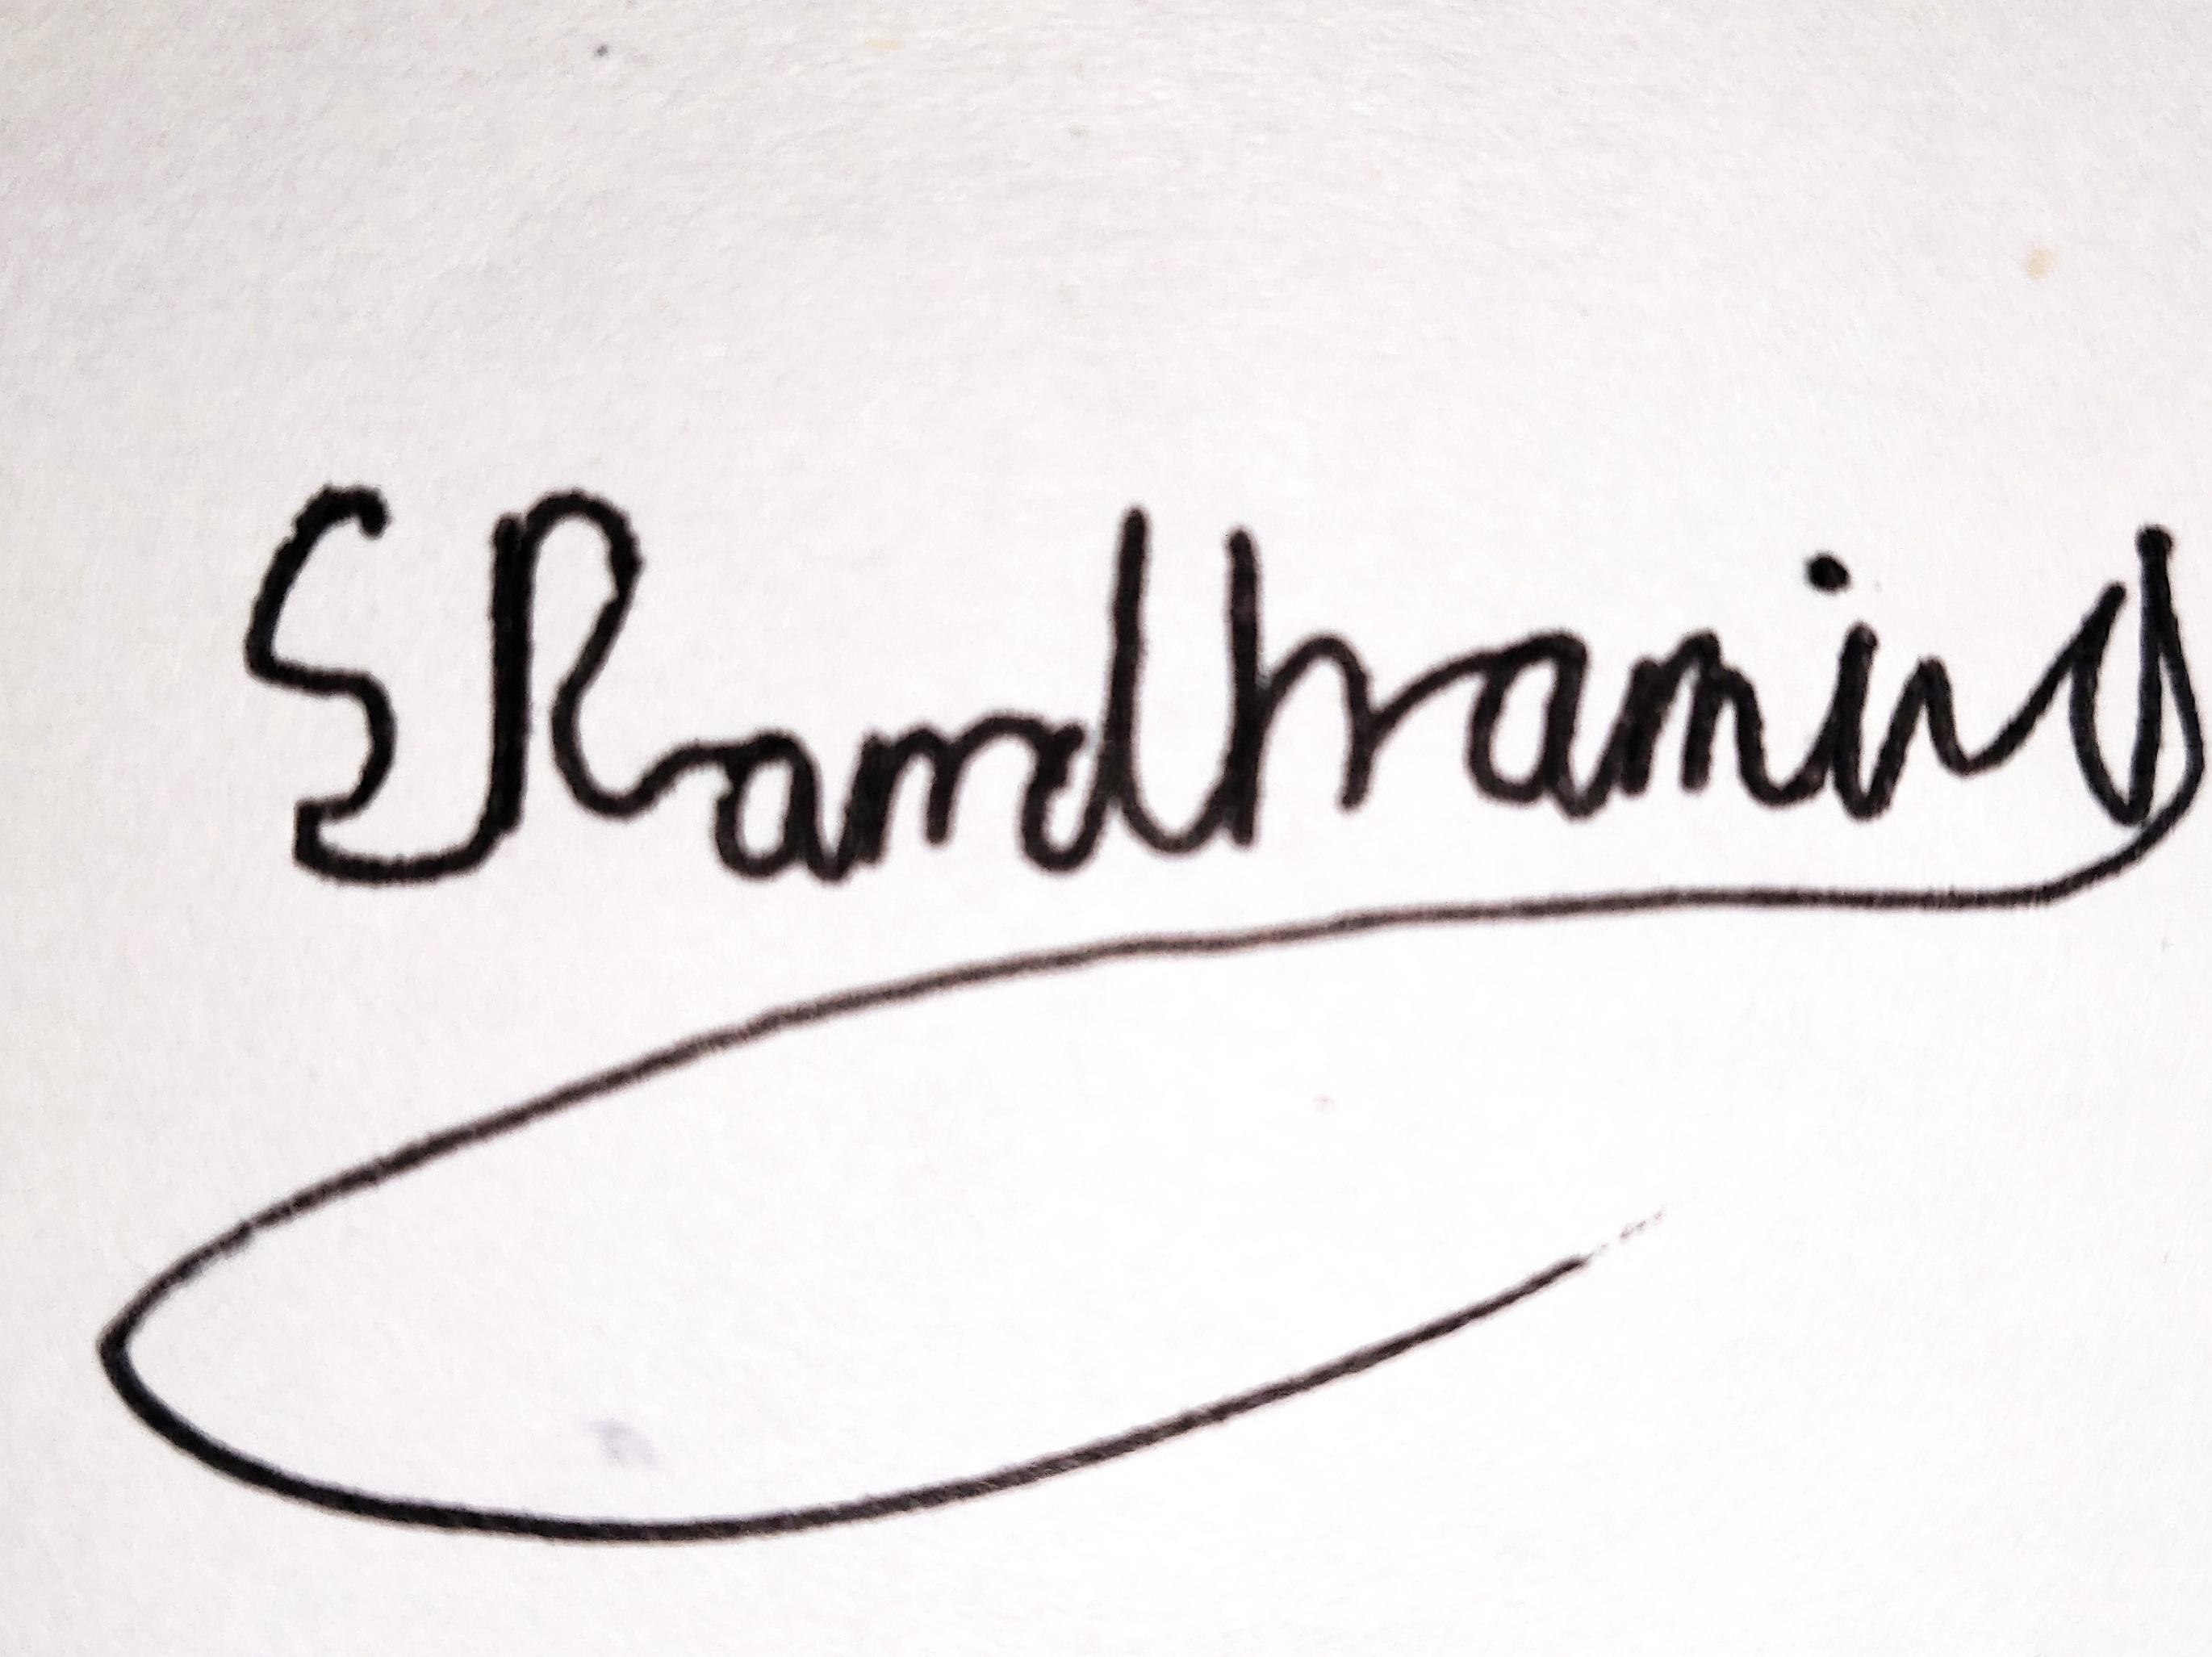
\includegraphics[scale=0.025]{logos/signature2.jpg}}................... DATE: .............\underline{\textbf{10/09/2020}}...................}
\end{quote}
\end{SingleSpace}
\clearpage
\clearemptydoublepage
%
\chapter*{Nomenclature}
    \begin{itemize}
        \item UAV - Unmanned Aerial Vehicle.
        \item GPS - Global Positioning System.
        \item LPS - Local Positioning System.
        \item FCU - Flight Controller Unit.
        \item UWB - Ultra-WideBand.
        \item TOF - Time of Flight.
        \item PSoC - Programmable System on Chip.
		\item NLOS - No Line of Sight.
		\item TWR - Two Way Ranging.
		\item I2C- Inter-Integrated Circuit Bus.
		\item SPI - Serial Peripheral Interface.
		\item OSH - Open-Source Hardware.
    \end{itemize}
\newpage
\renewcommand{\contentsname}{Table of Contents}
\maxtocdepth{subsection}
\tableofcontents*
\addtocontents{toc}{\par\nobreak \mbox{}\hfill{\bf Page}\par\nobreak}
\clearemptydoublepage
%
\listoftables
\addtocontents{lot}{\par\nobreak\textbf{{\scshape Table} \hfill Page}\par\nobreak}
\clearemptydoublepage
%
\listoffigures
\addtocontents{lof}{\par\nobreak\textbf{{\scshape Figure} \hfill Page}\par\nobreak}
\clearemptydoublepage
%
%
% The bulk of the document is delegated to these chapter files in
% subdirectories.
\mainmatter
%
%\import{chapters/chapter01/}{chap01.tex}
    \chapter{Introduction}\label{ch:introduction}
%    test ~\parencite{pozyx2018pozyx}
%    \lipsum[2-4]
    In recent years Unmanned aerial vehicle(UAV) usages has grown exponentially becoming common in industry and households~\parencite{custers2016drones}.
    A major part of UAV applications is their ability to localise themselves in the given environment with acceptable precision and accuracy.
    This is a common requirement in any robotic system but UAV's are often limited by strict payload requirements and therefore have to rely on sensors that are lightweight and robust.
    ~\textcite{ardupilotadvanced} gives a good summary of physical components that are used in various vehicles but a UAV system, specifically, a quadrotor system cab be summarised as follows:
    \begin{itemize}
        \item Rotor build - This section contains parts that should be researched based on the size and physical requirements of the drone.
        These include: brushless motors, electronic speed controllers, frame size.
        \item Flight controller unit(FCU) - This acts as the mother board and brain of the quadrotor system.
        It collates data from various sensors, sends commands to the motors and if there is a companion computer is attached collects and sends data to it.
        Commercial FCU's contain the various control systems and laws required for stable flight and movement.
        Most have an array of sensors built in.
        \item Sensors - These vary from from inertial, positioning, barometric and camera.
        Aside from inertial and barometric sensors that are present in most FCU's, sensors are chosen based on the environment and use case of the system.
        \item Companion computer - In some cases higher level processing is required by the system to execute autonomy and a secondary computer is used to do this.
        \item Transmitter and Receiver - This is used to implement manual control over the drone by a user.
    \end{itemize}
    Further delving into the sensors, we can classify UAV's based on their operating environment, indoors or outdoors.
    These give rise to two forms of localisation and navigation systems:
    \begin{itemize}
        \item Global Positioning Systems (GPS) - As the name suggests this setup uses GPS as well as other sensors.
        \item GPS-denied - These systems do not have access to GPS due to their operating environment.
    \end{itemize}
    In outdoor applications GPS provides a reliable and fairly accurate way to localise with use of several other sensors.
    However, indoor applications are denied the benefits of GPS and often must use other sensors for the task of localisation.
    Utilizing a similar concept of triangulation used by GPS a local positioning system(LPS) can be used for indoor environments.
    ~\textcite{pozyx2018pozyx} has developed a commercial system that utilizes Ultra-WideBand technology(UWB) with a bandwidth of $~\approx 500MHz$.

    With indoor environments users have more control of the environment so a LPS can create a feasible solution for indoor localisation for UAV's/robots operating there.
    The core idea of this research would be to integrate a commercial LPS directly into an existing FCU to produce accurate position estimates that can be used for autonomy.
    The measurements from the LPS would then be transformed into observations of the state of the UAV and fused with other observations from other sensors.
    This fused pose estimate would then be fed into the companion computer for off-board processing.
    \begin{figure}[h!]
        \centering
        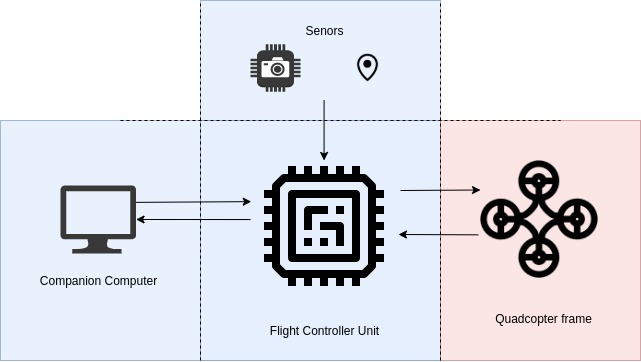
\includegraphics[scale=.65]{drone_setup}
        \caption{The typical setup for an autonomous UAV.}
        \label{fig:ds}
    \end{figure}

    Figure:~\ref{fig:ds} shows a typical setup for UAV.
    Parts of the system highlighted in blue represent systems that would be worked on during the course of this research.
    The idea is that the system being designed should provide localisation data which should be independent of the rotor build.
    These will be further scoped in the upcoming sections but it will involve doing a quality exercise of the LPS tp determine measurement uncertainty and limitations,
    writing additions or modifying the firmware of the FCU to integrate the LPS and setting up the piplines for a companion computer to receive the pose estimates and use them.



    % Give intro to LPS, proposed setup and then plan to complete

\section{Aims \& Objectives}\label{sec:aims_objs}

    In ~\ref{ch:intro} we briefly touched on what would be addressed over the course of this research.
Expanding on that, the research would entail the use of the commercial version of an UWB sensor for positioning from ~\cite{pozyx2018pozyx}.
At a high level the project and be split into three modules that must be researched, unit tested and finally integrated.
Figure ~\ref{fig:ds} highlights the major systems within the project and are as follows:
\begin{itemize}
    \item The Pozyx LPS providing measurements that will be used in localisation.
    \item A flight controller collating fusing various observations from sensors to provide a pose estimate.
    \item A companion computer to visualise and utilise the pose information in a meaningful manner.
\end{itemize}

From these systems and the overall aim of indoor localisation the following objectives were created:
\begin{itemize}
    \item Evaluation and qualitative analysis of the LPS, documentation limitations from previous done work and current physical setups as well as compare with other ranging standards.
    \item Based on the qualitative analysis and experiments determine the best configuration in a household to place the anchors for the system.
    \item Use the incoming data from the sensors to produce a suitable measurement/observation model for the pose of the system.
    \item Relay the data to a flight controller unit via a suitable hardware interface.
    \item Delve into the firmware of the flight controller and integrate the sensor readings into the codebase.
    \item Apply sensor fusion algorithms to provide pose estimates either onboard the flight controller or through some other medium.
    \item Evaluate pose estimates in various scenarios to see if they are viable for use.
\end{itemize}

All of these objectives can be completed without flying the UAV autonomously.
Given the current situation and time-frame it was determined that setting up the pipelines to visualise the localisation in realtime from the companion computer is adequate for the last objective.
Furthermore, with the autonomous flight being out of scope of this project much of the work fell into software engineering to achieve the overall aim.
Broadly, this means delving into the software libraries and interfaces for the Pozyx sensor, modifying and making additions to the Ardupilot flight stack to integrate the Pozyx sensor with the FCU,
and finally digging into the MAVLINK protocol and libraries to use the pose estimates on a Raspberry Pi 3 Model B+ PSoC.
To achieve these objectives a solid software engineering aproach would need to be applied with familiarity of Python and C++ programming languages.
Additionally, pose estimates should be evaluated under various tests which are not ideal for the LPS system to see how robust the estimator is.
A further limitation may be that due to the lack of accessible hardware and the scope of this research if pose estimates are unavailable from the flight controller a similar setup should be designed in order to closely emulate the results expected from the flight controller unit.


\section{Background Research}\label{sec:background}
Indoor localisation has become a core part of many systems in recent years.
These range from robotics, multimedia, logistics and sporting systems.
%Several modern localisation systems use signals and various analysis techniques to do positioning.
Modern localisation systems can be split into active or passive systems.
Active systems require the system being localised to have electronics to either process or send information that will be used to determine location.
In passive systems the position is determined  based on a variance of a measured signal or image data.
As noted by ~\cite{deak2012survey}, some of these techniques include, Received Signal Strength Indicator (RSSI), Time of Arrival (TOA), Time Difference of Arrival (TDOA) and Angle of Arrival (AOA).
The Pozyx commercial system uses UWB signals with a TOF technique in order to determine the position of a receiver (tag) in a network of transmitters (anchors).
Since processing is done on-board the tag, it falls under the active localisation category.
Active systems are ideal for indoor localisation systems for UAVs as the positional data can be fed directly to FCU's or companion computers in order to correct pose estimates.

As noted by the producers of Pozyx, the core of the system uses a communication bandwidth of $\approx 500M Hz$ which result in pulses of $0.16ns$ wide.
Assuming that speed of light is $299792458ms^-1$ we get pulses of length $0.04797m$ which is very small and hence robust to noise from reflections.
The major factors affecting the performance of the system would be materials that would slow down the signals before they reach the tag.
No Line of Sight (NLOS), conductors and changing mediums of travel are noted to affect the performance the most.

With the increasing complexity of FCU's it is possible to do relatively dense calculations in a real-time scenario without delegating them to a separate processing system.
This is beneficial to indoor drone systems since they need to be small and maneuverable.
A standard FCU comes equipped with several standard communication interfaces (I2C, Serial, SPI) so integrating external sensors is possible.
Furthermore, multiple autopilot firmware provides a Hardware Abstraction Layer (HAL) making any sensor integration developed on one unit easily ported to another system.
Additionally, onboard libraries contain sensor fusion implementations (Extended Kalman Filter (EKF)) that can combine the Pozyx data and on-board sensor data to provide fairly accurate positional data while in motion.
Given EKF's use in localisation, an alternative can be developed that can provide position estimates similar to what can be obtained from the FCU.
\chapter{Literature Review}\label{ch:literature-review}
\section{Indoor Localisation Systems}\label{sec:indoor-localisation-sensors}
\subsection*{Passive Systems}
In summary, passive systems do not require the object being tracked to have some of electronics on them to do positioning.
Some examples of passive systems are ~\citep{deak2012survey}:
\begin{itemize}
    \item Computer Vision and Imaging systems.
    \item Tactile and contact sensors.
    \item Attenuation of signals.
    \item Differential air pressure.
\end{itemize}
A common example of computer vision based localisation is to use a setup consisting of multiple cameras in a space trying to detecting a single object.
Using the intrinsic and extrinsic properties of each camera it is possible to determine the transform to the object in a given frame with relatively high accuracy.
A prime example of this is the commercial VICON motion capture systems.
~\cite{aerialrobotsiitk} shows a drone application in which the UAV is positioned via using a VICON motion capture system.
Figure~\ref{fig:vs} shows the simplified setup, it should be noted that the UAV must be equipped with specialised marker that is used to identify it.
Furthermore, the positions are fed to a companion computer connected to the autopilot system.
The VICON setup provides highly accurate positions and is often used to gather ground truth positional data to compare to other positioning systems.
The additional requirements of the VICON systems, however, do not make it feasible for indoor applications.

\begin{figure}[h!]
    \centering
    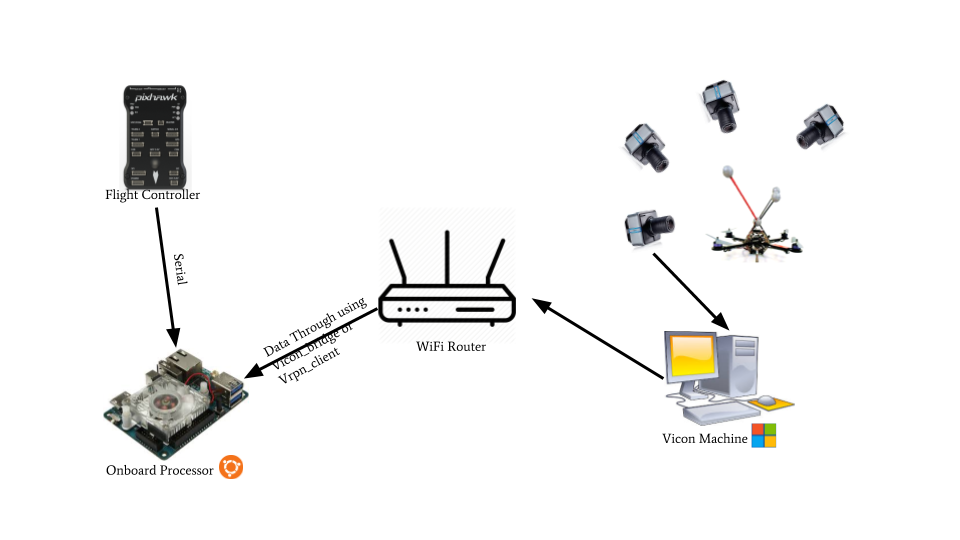
\includegraphics[scale=.45]{vicon_setup}
    \caption{VISON setup for position of a UAV. (\url{https://aerial-robotics-iitk.gitbook.io/wiki/estimation/setup-with-vicon})}
    \label{fig:vs}
\end{figure}

\subsection*{Active Systems}
In contrast to passive systems, active systems have the object being positioned equipped with electronics.
Many indoor localisation techniques use this and some examples are ~\cite{deak2012survey}
\begin{itemize}
    \item Radio-frequency identification
    \item UWB
    \item Wireless Local Area Network
    \item Bluetooth Low energy (BLE)
\end{itemize}
Many of these setups use an anchor and tag configuration.
The tag receives signals from multiple anchors and triangulates the tag.

An approach using and comparing UWB and BLE is developed by ~\cite{findobjs} to do localisation in a museum.
Both methods are combined with a dead reckoning system to improve accuracy.
Six paintings are equipped with both a BLE and UWB tag

\begin{figure}[h!]
    \centering
    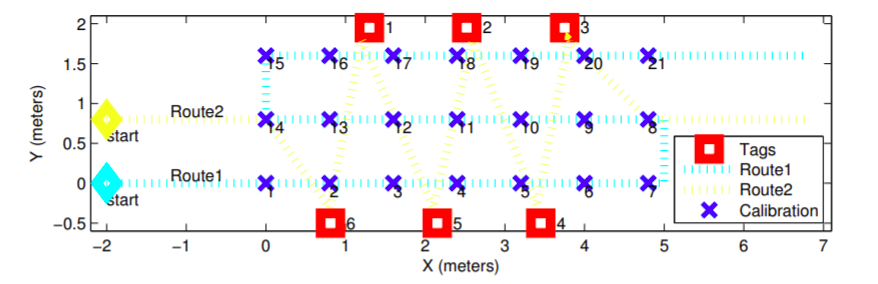
\includegraphics[scale=.45]{uwb_vs_ble}
    \caption{Setup used to compare UWB and BLE performance in a museum.}
    \label{fig:uwbvsble}
\end{figure}

\section{Pozyx - Behind the Scenes}\label{sec:pozyx---behind-the-scenes}

\chapter{Research Methodology}\label{ch:research-methodology}
%\lipsum[2-8]
\initial{F}rom the literature there is a clear lack of results for localisation systems using the commercial Pozyx sensor network with drones in an household environment.
To address the aims and objectives stated in ~\ref{sec:aims_objs}, it is proposed that a lightweight on-board localisation be developed to check the feasibility of minimal hardware solution for an indoor drone.
This would entail connecting a Pozyx tag directly to a FCU and integrate it with the pose localisation system existing already.
To close the loop the pose information should be available in some format that can be used for autonomous control.
Furthermore, the system should be tested in a practical environment, to this end, the Pozyx anchor network was setup in a kitchen.
A kitchen represents one of the highest traffic areas in a household and it contains various materials that will make raw readings from a UWB system noisy and inaccurate.
As a kitchen will contain both dynamic and static obstacles multiple anchor configurations must be tested in order to find optimal anchor positions in this given environment.

\section{Anchor Configurations}\label{sec:anchor-configurations}
Noting work from ~\citet{di2019evaluation} and the setup procedures from ~\citet{pozyx2018pozyx} it is important to have at least 4 anchors setup in non-planar orientations for the best positioning results.
To determine a suitable anchor configuration in the given space a tag was placed at fixed known point in a given reference frame and the mounted locations of the 4 anchors were varied on each wall of the kitchen in order to prevent planar configurations and ambiguity when the tag calculates its position.
Figure ~\ref{fig:layout} shows a simplified layout and toybox configuration of the tag and anchors.
Grey areas represent areas in the space that is impossible to traverse, red represents known obstacles that interfere and attenuate the UWB signal, blue represent anchors, green the tag, cream is partially obstructed and the rest of the area is fully traversable.
Before each run and data collection the tag was manually configured with the location of each of the anchors in the reference frame of the kitchen and recorded for at least 5 seconds.
The tag was triggered to calculate the position repeatedly within the timeframe and the function call is blocking and takes $\approx70ms$ so data was recorded at a frequency of $\approx14.28Hz$.
With a tag position of (1480,2330,980)mm, the following statistics were calculated using Matlab.
In addition to the average error and standard deviation,  kurtosis and skew metrics were added to show the number of outliers and symmetry of the recorded data.
The error metrics are important to give an idea of how noisy the overall data is while kurtosis and skewness gives an indication if the noise follows a uniform distribution which would be beneficial ideal for state estimators.
From table ~\ref{tb:config_stats} we can see that configuration 12 gives acceptable error metrics and reasonable skew and kurtosis making it the best out of the configurations tested.
To further support this Figure ~\ref{fig:config} shows several results obtained with several configurations and it can be seen that configuration 12 produced the best results.

\begin{figure}[h!]
    \centering
    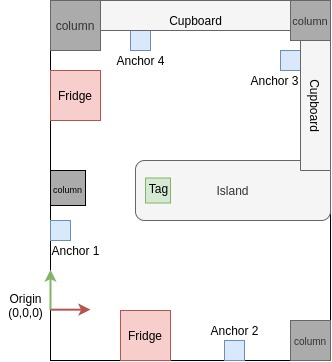
\includegraphics{mtd/Kitchen_layout}
    \caption{Birds eye view of the test environment.}
    \label{fig:layout}
\end{figure}
\newpage
%\begin{table}[h!]
   \begin{longtable}[h!]{| c | c | c | c | c | c |}
       \hline
       Config \#& Anchor positions (mm)
       & Avg. Error & Std. Deviation$\left(\begin{array}{c}
       x,\\y,\\z
       \end{array}\right)$ & Kurtosis & Skewness\\
       \hline
       1 & $\left(\begin{array}{c}
       (0,0,1115),\\(3680, -405, 1550),\\(3655, 4080, 1906),\\(270, 4465, 2090)
       \end{array}\right)$& 342.5906 & $\left(\begin{array}{c}
       183.1707,\\205.3426,\\972.6239
       \end{array}\right)$&$\left( \begin{array}{c}
       2.349,\\ 1.5967,\\ 1.415
       \end{array} \right)$&$\left( \begin{array}{c}
       -0.4083,\\ -0.3522,\\ 0.4551
       \end{array} \right)$\\
       \hline
              2 & $\left(\begin{array}{c}
       (0,665,1115),\\(2995, -405, 1889),\\(3655, 4080, 1906),\\(270, 4465, 2090)
       \end{array}\right)$& 173.5938 & $\left(\begin{array}{c}
       43.2345,\\45.6897,\\133.8616\\
       \end{array}\right)$&$\left( \begin{array}{c}
       21.8923,\\ 10.1765,\\ 119.1344
       \end{array} \right)$&$\left( \begin{array}{c}
       -2.8672,\\ -0.3453,\\ 8.9025
       \end{array} \right)$\\
       \hline
              3 & $\left(\begin{array}{c}
       (0,665,1115),\\(2995, -405, 1889),\\(3655, 4080, 1906),\\(1526, 4559, 837)
       \end{array}\right)$& 203.8502 & $\left(\begin{array}{c}
       128.4693,\\118.3216,\\209.1637
       \end{array}\right)$&$\left( \begin{array}{c}
       14.2955,\\ 11.2045,\\ 2.9124
       \end{array} \right)$&$\left( \begin{array}{c}
       -2.579,\\  -0.3920,\\ 0.4055
       \end{array} \right)$\\
       \hline
              4 & $\left(\begin{array}{c}
       (0,665,1115),\\(2995, -405, 1889),\\(3655, 4080, 1906),\\(1070, 5170, 491)
       \end{array}\right)$& 85.8562 & $\left(\begin{array}{c}
       40.2197,\\40.6081,\\66.2120
       \end{array}\right)$&$\left( \begin{array}{c}
       6.7558,\\ 7.5180,\\ 3.4722
       \end{array} \right)$&$\left( \begin{array}{c}
       -0.4260,\\ -0.5344,\\ -0.1242
       \end{array} \right)$\\
       \hline
              5 & $\left(\begin{array}{c}
       (0,665,1115),\\(2995, -405, 1889),\\(3960, 3368, 2304),\\(1070, 5170, 491)
       \end{array}\right)$& 64.8616 & $\left(\begin{array}{c}
       65.3883,\\53.8458,\\78.5751
       \end{array}\right)$&$\left( \begin{array}{c}
       13.3707,\\ 13.2178,\\ 11.0111
       \end{array} \right)$&$\left( \begin{array}{c}
       -0.6016,\\ 0.3745,\\ 0.0461
       \end{array} \right)$\\
       \hline
              6 & $\left(\begin{array}{c}
       (0,665,1115),\\(2737, -410, 1913),\\(3655, 3598, 1668),\\(1187, 4760, 590)
       \end{array}\right)$& 189.933 & $\left(\begin{array}{c}
       40.8435,\\32.6482,\\58.5618
       \end{array}\right)$&$\left( \begin{array}{c}
       11.8957,\\ 11.8924,\\ 11.092
       \end{array} \right)$&$\left( \begin{array}{c}
       0.7516,\\ -0.0100,\\ -0.1322
       \end{array} \right)$\\
       \hline
              7 & $\left(\begin{array}{c}
       (0,665,1115),\\(2737, -410, 1913),\\(3655, 4529, 1777),\\(1187, 4760, 590)
       \end{array}\right)$& 100.6929 & $\left(\begin{array}{c}
       75.8269,\\72.0940,\\41.9398
       \end{array}\right)$&$\left( \begin{array}{c}
       26.0285,\\ 17.4295,\\ 7.2328
       \end{array} \right)$&$\left( \begin{array}{c}
       -3.1681,\\ -0.8384,\\ -0.7151
       \end{array} \right)$\\
       \hline
              8 & $\left(\begin{array}{c}
       (0,645,1214),\\(2737, -410, 1913),\\(3651, 4120, 1853),\\(1066, 4760, 491)
       \end{array}\right)$& 138.1276 & $\left(\begin{array}{c}
       26.2243,\\21.8750,\\70.6189
       \end{array}\right)$&$\left( \begin{array}{c}
       4.6048,\\ 52.2374,\\ 50.9467
       \end{array} \right)$&$\left( \begin{array}{c}
       -0.4858,\\ 5.0752,\\ 5.1757
       \end{array} \right)$\\
       \hline
              9 & $\left(\begin{array}{c}
       (0,645,1214),\\(2737, -410, 1913),\\(3970, 3063, 2320),\\(1066, 4760, 491)
       \end{array}\right)$& 258.296 & $\left(\begin{array}{c}
       165.7105,\\95.081,\\475.0623
       \end{array}\right)$&$\left( \begin{array}{c}
       2.2833,\\ 1.7939,\\ 2.3406
       \end{array} \right)$&$\left( \begin{array}{c}
       -0.6982,\\ 0.2746,\\ 0.7517
       \end{array} \right)$\\
       \hline
              10 & $\left(\begin{array}{c}
       (0,645,1214),\\(2737, -410, 1913),\\(3651, 3550, 1810),\\(1066, 4760, 491)
       \end{array}\right)$& 235.348 & $\left(\begin{array}{c}
       116.1306,\\89.9868,\\420.8322
       \end{array}\right)$&$\left( \begin{array}{c}
       3.6670,\\ 4.7058,\\ 3.8066
       \end{array} \right)$&$\left( \begin{array}{c}
       1.5079,\\ -1.7613,\\ -1.5615
       \end{array} \right)$\\
       \hline
              11 & $\left(\begin{array}{c}
       (0,645,1214),\\(2737, -410, 1913),\\(3651, 3550, 1810),\\(1591, 4450, 1775)
       \end{array}\right)$& 223.4468 & $\left(\begin{array}{c}
       120.9674,\\79.8602,\\409.8192
       \end{array}\right)$&$\left( \begin{array}{c}
       3.389,\\ 4.6663,\\ 3.1988
       \end{array} \right)$&$\left( \begin{array}{c}
       1.1099,\\ -1.5397,\\ -1.2038
       \end{array} \right)$\\
       \hline
              12 & $\left(\begin{array}{c}
       (0,645,1214),\\(2737, -410, 1913),\\(3651, 4120, 1853),\\(1591, 4450, 1775)
       \end{array}\right)$& 111.8493 & $\left(\begin{array}{c}
       27.568,\\17.7124,\\64.4278
       \end{array}\right)$&$\left( \begin{array}{c}
       4.8522,\\ 7.4335,\\ 6.2489
       \end{array} \right)$&$\left( \begin{array}{c}
       -0.0239,\\ -0.8535,\\ 3.7132
       \end{array} \right)$\\
       \hline
       \caption{Statistics of the data recorded for each configuration.}
        \label{tb:config_stats}
   \end{longtable}
%\end{table}

    \begin{figure}[h!]
        \centering
        \begin{subfigure}[b]{0.49\textwidth}
            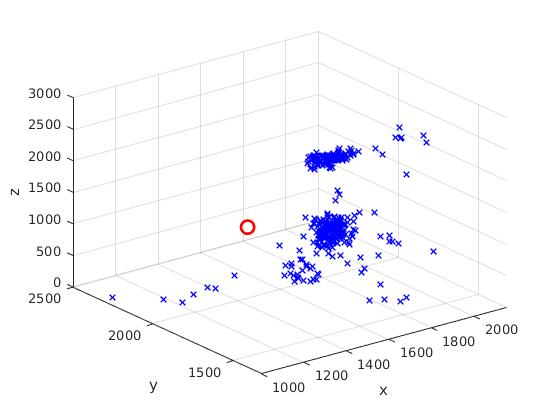
\includegraphics[width=\textwidth]{results/config1}
            \caption{Plot of Config 1}
        \end{subfigure}
        ~ %add desired spacing between images, e. g. ~, \quad, \qquad, \hfill etc.
          %(or a blank line to force the subfigure onto a new line)
        \begin{subfigure}[b]{0.49\textwidth}
            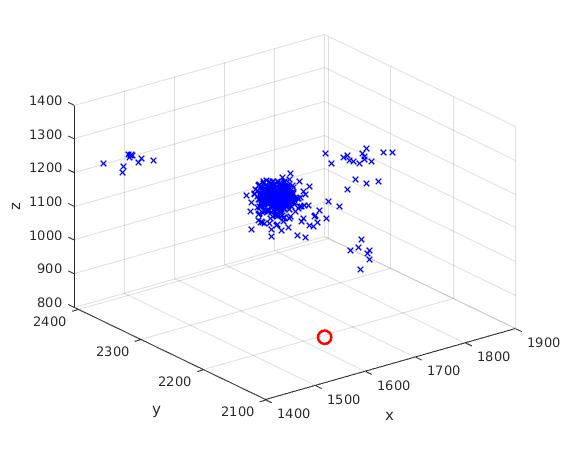
\includegraphics[width=\textwidth]{results/config6}
            \caption{Plot of Config 6}
        \end{subfigure}

        \begin{subfigure}[b]{\textwidth}
            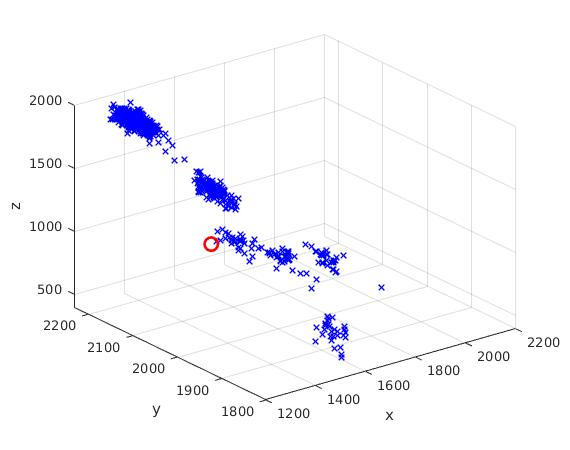
\includegraphics[width=\textwidth]{results/config11}
            \caption{Plot of Config 12}
        \end{subfigure}
        \caption{Sample plots of several anchor configurations.}
        \label{fig:config}
    \end{figure}

%TODO: Insert the pics I took of the anchors here.
Intro to the basic concept, highlight Pietra's paper and how I am using that to phrase and determine the best location
Show pics, diagrams and initial table of results?

\clearemptydoublepage
%
%
% And the appendix goes here
\appendix
\import{chapters/appendices/}{app0A.tex}
\clearemptydoublepage
%
% Apparently the guidelines don't say anything about citations or
% bibliography styles so I guess we can use anything.
\backmatter
\bibliographystyle{agsm}
\refstepcounter{chapter}
\bibliography{thesisbiblio}
\clearemptydoublepage
%
% Add index
%\printindex
%   
\end{document}